% !TeX root = ../main.tex

\chapter{Resultados}

  \section{Requerimientos}
  % en esta seccion requerimos a las historias de usuario para  tal explicar que es un hiustoria de usuario y poner la tabla de excel, despues lo de los riesgos y tamhbien la tabla
  %poner subseccion de hu, y otra de doc de riesgos el de hu mira se tratara estos temas desde perspectiva de usaurios de lo que puede y que no

  %primer parrafo explicar que se usaron HU y doc de riesgos ya que hace parte de rup
  %+++++++
  %vendria a ser inicio

  %definir las hu, pero sin las columnas de epicas ni de priroidad

  %identificar riesgos, tabla de riesgos pues los primeras tres columnas hasta causa

  %planificar fase de elaboración, pondremos mucho texto inventado y ya, sobre lo de que decidimos usar estas HU porque tal y cosas asi

  En esta sección se presentan los artefactos generados durante la fase de inicio del proyecto siguiendo la metodología propuesta. Estos artefactos son una primera versión de lo que se fue iterando durante el desarrollo de las actividades definidas.\\
  A continuación, se detallan las historias de usuario (HU) que definen los requerimientos funcionales, así como la matriz de riesgos que identifica y evalúa los posibles obstáculos que podría haber afectado el desarrollo del videojuego serio.



  \subsection{Historias de Usuario}


  Se empezó escribiendo la HU en base a las ideas principales y las mecánicas básicas, después se empezó modificar y/o crear ciertas HU dirigidos a cumplir con los aspectos escenciales para considerar el videojuego como un GBL.\\
  La primera iteración de las HU se redactaron en una tabla simple que contenía únicamente el código y la descripción de cada historia.
  Esta versión inicial sirvió como base para identificar las funcionalidades clave del sistema y establecer un marco de referencia para el desarrollo posterior.
  La Tabla \ref{tab:hu-inicial} muestra las historias de usuario definidas en la primera iteración.

\begin{longtable}{|c|L{12cm}|}
\caption{Primera versión de las Historias de Usuario} \label{tab:hu-inicial} \\
\hline
\textbf{Código} & \textbf{Historia de Usuario} \\ \hline
\endfirsthead

\hline
\textbf{Código} & \textbf{Historia de Usuario} \\ \hline
\endhead

\hline
\multicolumn{2}{r}{\textit{Continúa en la siguiente página}} \\
\endfoot

\hline
\endlastfoot
HU1 & Como jugador, quiero ver una pantalla de selección de niveles para elegir cuál jugar  \\ \hline
HU2 & Como jugador, quiero que al empezar un nivel, se me presente una pantalla de contrato que detalle el presupuesto, los objetivos y los posibles desafíos \\ \hline
HU3 & Como jugador, quiero poder mover la cámara (panorámica) por el mapa para explorar el terreno \\ \hline
HU4 & Como jugador, quiero poder acercar y alejar la vista (zoom) para ver el mapa con diferentes niveles de detalle \\ \hline
HU5 & Como jugador, quiero ver las delimitaciones políticas y ríos \\ \hline
HU6 & Como jugador, quiero ver un terreno del nivel a jugar \\ \hline
HU7 & Como jugador, quiero poder rotar la cámara para observar el terreno desde distintos ángulos \\ \hline
HU8 & Como jugador, quiero poder activar una capa de eventos para visualizar las zonas de riesgo y planificar mi ruta en consecuencia \\ \hline
HU9 & Como jugador, quiero poder construir un tramo de vía férrea entre dos puntos \\ \hline
HU10 & Como jugador, quiero poder eliminar un tramo de vía férrea para rediseñar mis rutas \\ \hline
HU11 & Como jugador, quiero que se pueda construya un puente o valles \\ \hline
HU12 & Como jugador, quiero que se construya automáticamente un túnel si mi vía férrea atraviesa una montaña \\ \hline
HU13 & Como jugador, quiero poder construir estaciones en puntos específicos de la vía para definir los puntos de inicio y fin del ciclo \\ \hline
HU14 & Como jugador, quiero que la interfaz muestre mi presupuesto actual en todo momento para controlar mis gastos de construcción \\ \hline
HU15 & Como jugador, quiero poder deshacer mi última acción de construcción para corregir un error rápidamente \\ \hline
HU16 & Como jugador, tras diseñar la ruta, quiero acceder a un menú para seleccionar y comprar la locomotora que usaré \\ \hline
HU17 & Como jugador, quiero poder añadir vagones específicos (pasajeros, carga) a mi locomotora para cumplir los requisitos del contrato \\ \hline
HU18 & Como jugador, quiero que el menú de selección me muestre las locomotoras de la ruta que diseñé \\ \hline
HU19 & Como jugador, durante la simulación, quiero ver una alerta o efecto visual cuando un tren está sufriendo daños al pasar por una zona de evento \\ \hline
HU20 & Como jugador, quiero que el botón de "Hacer Testeo" me informe si me falta algún requisito para iniciar la simulación \\ \hline
HU21 & Como jugador, quiero tener la opción de volver a la fase de construcción después de un testeo para modificar mis rutas antes de la evaluación final \\ \hline
HU22 & Como jugador, al finalizar un nivel, quiero ver una pantalla de puntuación que califique mi desempeño \\ \hline
HU23 & Como jugador, quiero que mi puntuación final considere la rentabilidad (costo total vs. valor del contrato) \\ \hline
HU24 & Como jugador, quiero que mi puntuación final considere la durabilidad (estado final de mis trenes y vías tras la simulación) \\ \hline
HU25 & Como jugador, quiero que mi puntuación final considere la eficiencia (tiempo que tardó el tren en completar el ciclo) \\ \hline
HU26 & Como jugador, quiero ver un informe detallado que desglose mi puntuación final para entender cómo mejorar \\ \hline
HU27 & Como jugador, quiero que se desbloqueen nuevos niveles en el menú de selección tras completar el contrato actual \\ \hline
HU28 & Como jugador, quiero que Don Raíl me presente el contrato al inicio de cada nivel con un diálogo breve, para darme un objetivo narrativo y contexto histórico sobre la región \\ \hline
HU29 & Como nuevo jugador, quiero que Don Raíl me guíe a través de un tutorial interactivo en el primer nivel, para aprender las mecánicas del juego de una forma amigable y contextual \\ \hline
HU30 & Como jugador, quiero que Don Raíl me dé una advertencia contextual si construyo una vía con una pendiente muy pronunciada o una curva muy cerrada, para que pueda corregir errores de ingeniería antes del testeo \\ \hline
HU31 & Como jugador, quiero que al seleccionar una estación o ciudad importante, aparezca un ícono de Don Raíl que pueda clickear para escuchar un dato histórico sobre la importancia ferroviaria de ese lugar \\ \hline
HU32 & Como jugador, quiero escuchar o leer un breve comentario de Don Raíl cuando un tren sufre un evento durante la simulación, para aumentar la inmersión \\ \hline
HU33 & Como jugador, quiero que Don Raíl comente sobre mi puntuación final, celebrando el éxito con emoción o dándome un consejo en caso de fallar para que la evaluación se sienta más personal \\ \hline
HU34 & Como jugador, quiero que durante las pantallas de carga, aparezcan anécdotas cortas o "dichos" de Don Raíl sobre la vida en el ferrocarril, para enriquecer el mundo del juego y aprovechar los tiempos de espera \\ \hline
HU35 & Como administrador, quiero adquirir y guardar metadatos de los jugadores en una base de datos para poder generar informes \\ \hline
\end{longtable}

\section{Diseño}
% (Completar) vendria a ser elaboracion
% organizar las HU?
osea poner lo que esta en la columna de epica, quitar la prioridad, eso de M S C
% explicar epicas tambien la tabla de epicas
\subsection{Organización de las HU}
Para organizar el desarrollo del proyecto, se definieron un conjunto de épicas que agrupan las principales funcionalidades del sistema.
Estas sirvieron como base para clasificar las historias de usuario y facilitar la planificación y el seguimiento del avance.
En la Cuadro \ref{tab:épicas} se presentan las épicas establecidas para el proyecto cada una enumerada para la futura agrupación de historias de usuario.
\begin{table}[H] \centering \caption{Épicas} \label{tab:épicas} 
\begin{tabular}{|c|l|} 
\hline \textbf{Épica} & \textbf{Nombre}\\ \hline 
1 & Selección de Nivel y Contratos \\ \hline 
2 & Interacción con el Mapa 3D \\ \hline 
3 & Sistema de Construcción de Vías \\ \hline 
4 & Gestión de Material Rodante \\ \hline 
5 & Motor de Simulación y Eventos \\ \hline 
6 & Sistema de Evaluación y Puntuación \\ \hline 
7 & Progresión y Rejugabilidad \\ \hline 
8 & Narrativa y Mentoría\\ \hline 
\end{tabular} 
\end{table}

Una vez definidas, se procedió a asignar cada épica a la historia de usuario correspondiente, de acuerdo con la funcionalidad o el componente 
del sistema al que contribuía. Esta clasificación permitió identificar con claridad el subsistema o área funcional a la que pertenecía cada historia, favoreciendo una organización más coherente del desarrollo y una mejor comprensión del alcance de cada módulo dentro del proyecto.
\begin{longtable}{|c|c|L{10cm}|}
\caption{Historias de Usuario} \label{tab:hu} \\
\hline
\textbf{Épica} & \textbf{Código} & \textbf{Historia de Usuario} \\ \hline
\endfirsthead

\hline
\textbf{Épica} & \textbf{Código} & \textbf{Historia de Usuario} \\ \hline
\endhead

\hline
\multicolumn{3}{r}{\textit{Continúa en la siguiente página}} \\
\endfoot

\hline
\endlastfoot
1 & HU1 & Como jugador, quiero ver una pantalla de selección de niveles para elegir cuál jugar  \\ \hline
1 & HU2 & Como jugador, quiero que al empezar un nivel, se me presente una pantalla de contrato que detalle el presupuesto, los objetivos y los posibles desafíos \\ \hline
2 & HU3 & Como jugador, quiero poder mover la cámara (panorámica) por el mapa para explorar el terreno \\ \hline
2 & HU4 & Como jugador, quiero poder acercar y alejar la vista (zoom) para ver el mapa con diferentes niveles de detalle \\ \hline
2 & HU5 & Como jugador, quiero ver las delimitaciones políticas y ríos \\ \hline
2 & HU6 & Como jugador, quiero ver un terreno del nivel a jugar \\ \hline
2 & HU7 & Como jugador, quiero poder rotar la cámara para observar el terreno desde distintos ángulos \\ \hline
2 & HU8 & Como jugador, quiero poder activar una capa de eventos para visualizar las zonas de riesgo y planificar mi ruta en consecuencia \\ \hline
3 & HU9 & Como jugador, quiero poder construir un tramo de vía férrea entre dos puntos \\ \hline
3 & HU10 & Como jugador, quiero poder eliminar un tramo de vía férrea para rediseñar mis rutas \\ \hline
3 & HU11 & Como jugador, quiero que se pueda construya un puente o valles \\ \hline
3 & HU12 & Como jugador, quiero que se construya automáticamente un túnel si mi vía férrea atraviesa una montaña \\ \hline
3 & HU13 & Como jugador, quiero poder construir estaciones en puntos específicos de la vía para definir los puntos de inicio y fin del ciclo \\ \hline
3 & HU14 & Como jugador, quiero que la interfaz muestre mi presupuesto actual en todo momento para controlar mis gastos de construcción \\ \hline
3 & HU15 & Como jugador, quiero poder deshacer mi última acción de construcción para corregir un error rápidamente \\ \hline
4 & HU16 & Como jugador, tras diseñar la ruta, quiero acceder a un menú para seleccionar y comprar la locomotora que usaré \\ \hline
4 & HU17 & Como jugador, quiero poder añadir vagones específicos (pasajeros, carga) a mi locomotora para cumplir los requisitos del contrato \\ \hline
4 & HU18 & Como jugador, quiero que el menú de selección me muestre las locomotoras de la ruta que diseñé \\ \hline
5 & HU19 & Como jugador, durante la simulación, quiero ver una alerta o efecto visual cuando un tren está sufriendo daños al pasar por una zona de evento \\ \hline
5 & HU20 & Como jugador, quiero que el botón de "Hacer Testeo" me informe si me falta algún requisito para iniciar la simulación \\ \hline
5 & HU21 & Como jugador, quiero tener la opción de volver a la fase de construcción después de un testeo para modificar mis rutas antes de la evaluación final \\ \hline
6 & HU22 & Como jugador, al finalizar un nivel, quiero ver una pantalla de puntuación que califique mi desempeño \\ \hline
6 & HU23 & Como jugador, quiero que mi puntuación final considere la rentabilidad (costo total vs. valor del contrato) \\ \hline
6 & HU24 & Como jugador, quiero que mi puntuación final considere la durabilidad (estado final de mis trenes y vías tras la simulación) \\ \hline
6 & HU25 & Como jugador, quiero que mi puntuación final considere la eficiencia (tiempo que tardó el tren en completar el ciclo) \\ \hline
6 & HU26 & Como jugador, quiero ver un informe detallado que desglose mi puntuación final para entender cómo mejorar \\ \hline
7 & HU27 & Como jugador, quiero que se desbloqueen nuevos niveles en el menú de selección tras completar el contrato actual \\ \hline
7 & HU28 & Como jugador, quiero que Don Raíl me presente el contrato al inicio de cada nivel con un diálogo breve, para darme un objetivo narrativo y contexto histórico sobre la región \\ \hline
8 & HU29 & Como nuevo jugador, quiero que Don Raíl me guíe a través de un tutorial interactivo en el primer nivel, para aprender las mecánicas del juego de una forma amigable y contextual \\ \hline
8 & HU30 & Como jugador, quiero que Don Raíl me dé una advertencia contextual si construyo una vía con una pendiente muy pronunciada o una curva muy cerrada, para que pueda corregir errores de ingeniería antes del testeo \\ \hline
8 & HU31 & Como jugador, quiero que al seleccionar una estación o ciudad importante, aparezca un ícono de Don Raíl que pueda clickear para escuchar un dato histórico sobre la importancia ferroviaria de ese lugar \\ \hline
8 & HU32 & Como jugador, quiero escuchar o leer un breve comentario de Don Raíl cuando un tren sufre un evento durante la simulación, para aumentar la inmersión \\ \hline
8 & HU33 & Como jugador, quiero que Don Raíl comente sobre mi puntuación final, celebrando el éxito con emoción o dándome un consejo en caso de fallar para que la evaluación se sienta más personal \\ \hline
8 & HU34 & Como jugador, quiero que durante las pantallas de carga, aparezcan anécdotas cortas o "dichos" de Don Raíl sobre la vida en el ferrocarril, para enriquecer el mundo del juego y aprovechar los tiempos de espera \\ \hline
6 & HU35 & Como administrador, quiero adquirir y guardar metadatos de los jugadores en una base de datos para poder generar informes \\ \hline
\end{longtable}

%colocar capturas de los primeros intentos
%capturas de los videos con explicaciones de que tanto se hacia y el como fue la adaptacion, entre esos mencionando el que el mapa antiguo estaba mal y porque y todo eso
\subsection{Elaboración de la maqueta}

\subsubsection{Terreno}
La primera maqueta a realizar se trataba del principal entorno de interacción que tendrá el jugador con el entorno, en este caso, el mapa en 3 dimensiones de Colombia.
Para eso, se realizó un modelado en \textit{Blender} utilizando una técnica de elevación por textura, en la cual se empleó una imagen en escala de grises para representar las variaciones de altura del terreno (DEM).
Dicha imagen, de resolución limitada, permitió obtener un modelo base del relieve, aunque con una precisión reducida debido a la baja calidad del mapa de elevación.
En la Figura \ref{fig:mapa-altura} se presenta la textura empleada y el resultado del modelo tridimensional generado a partir de ella.
\begin{figure}[H]
\centering
\begin{minipage}{0.45\textwidth}
    \centering
    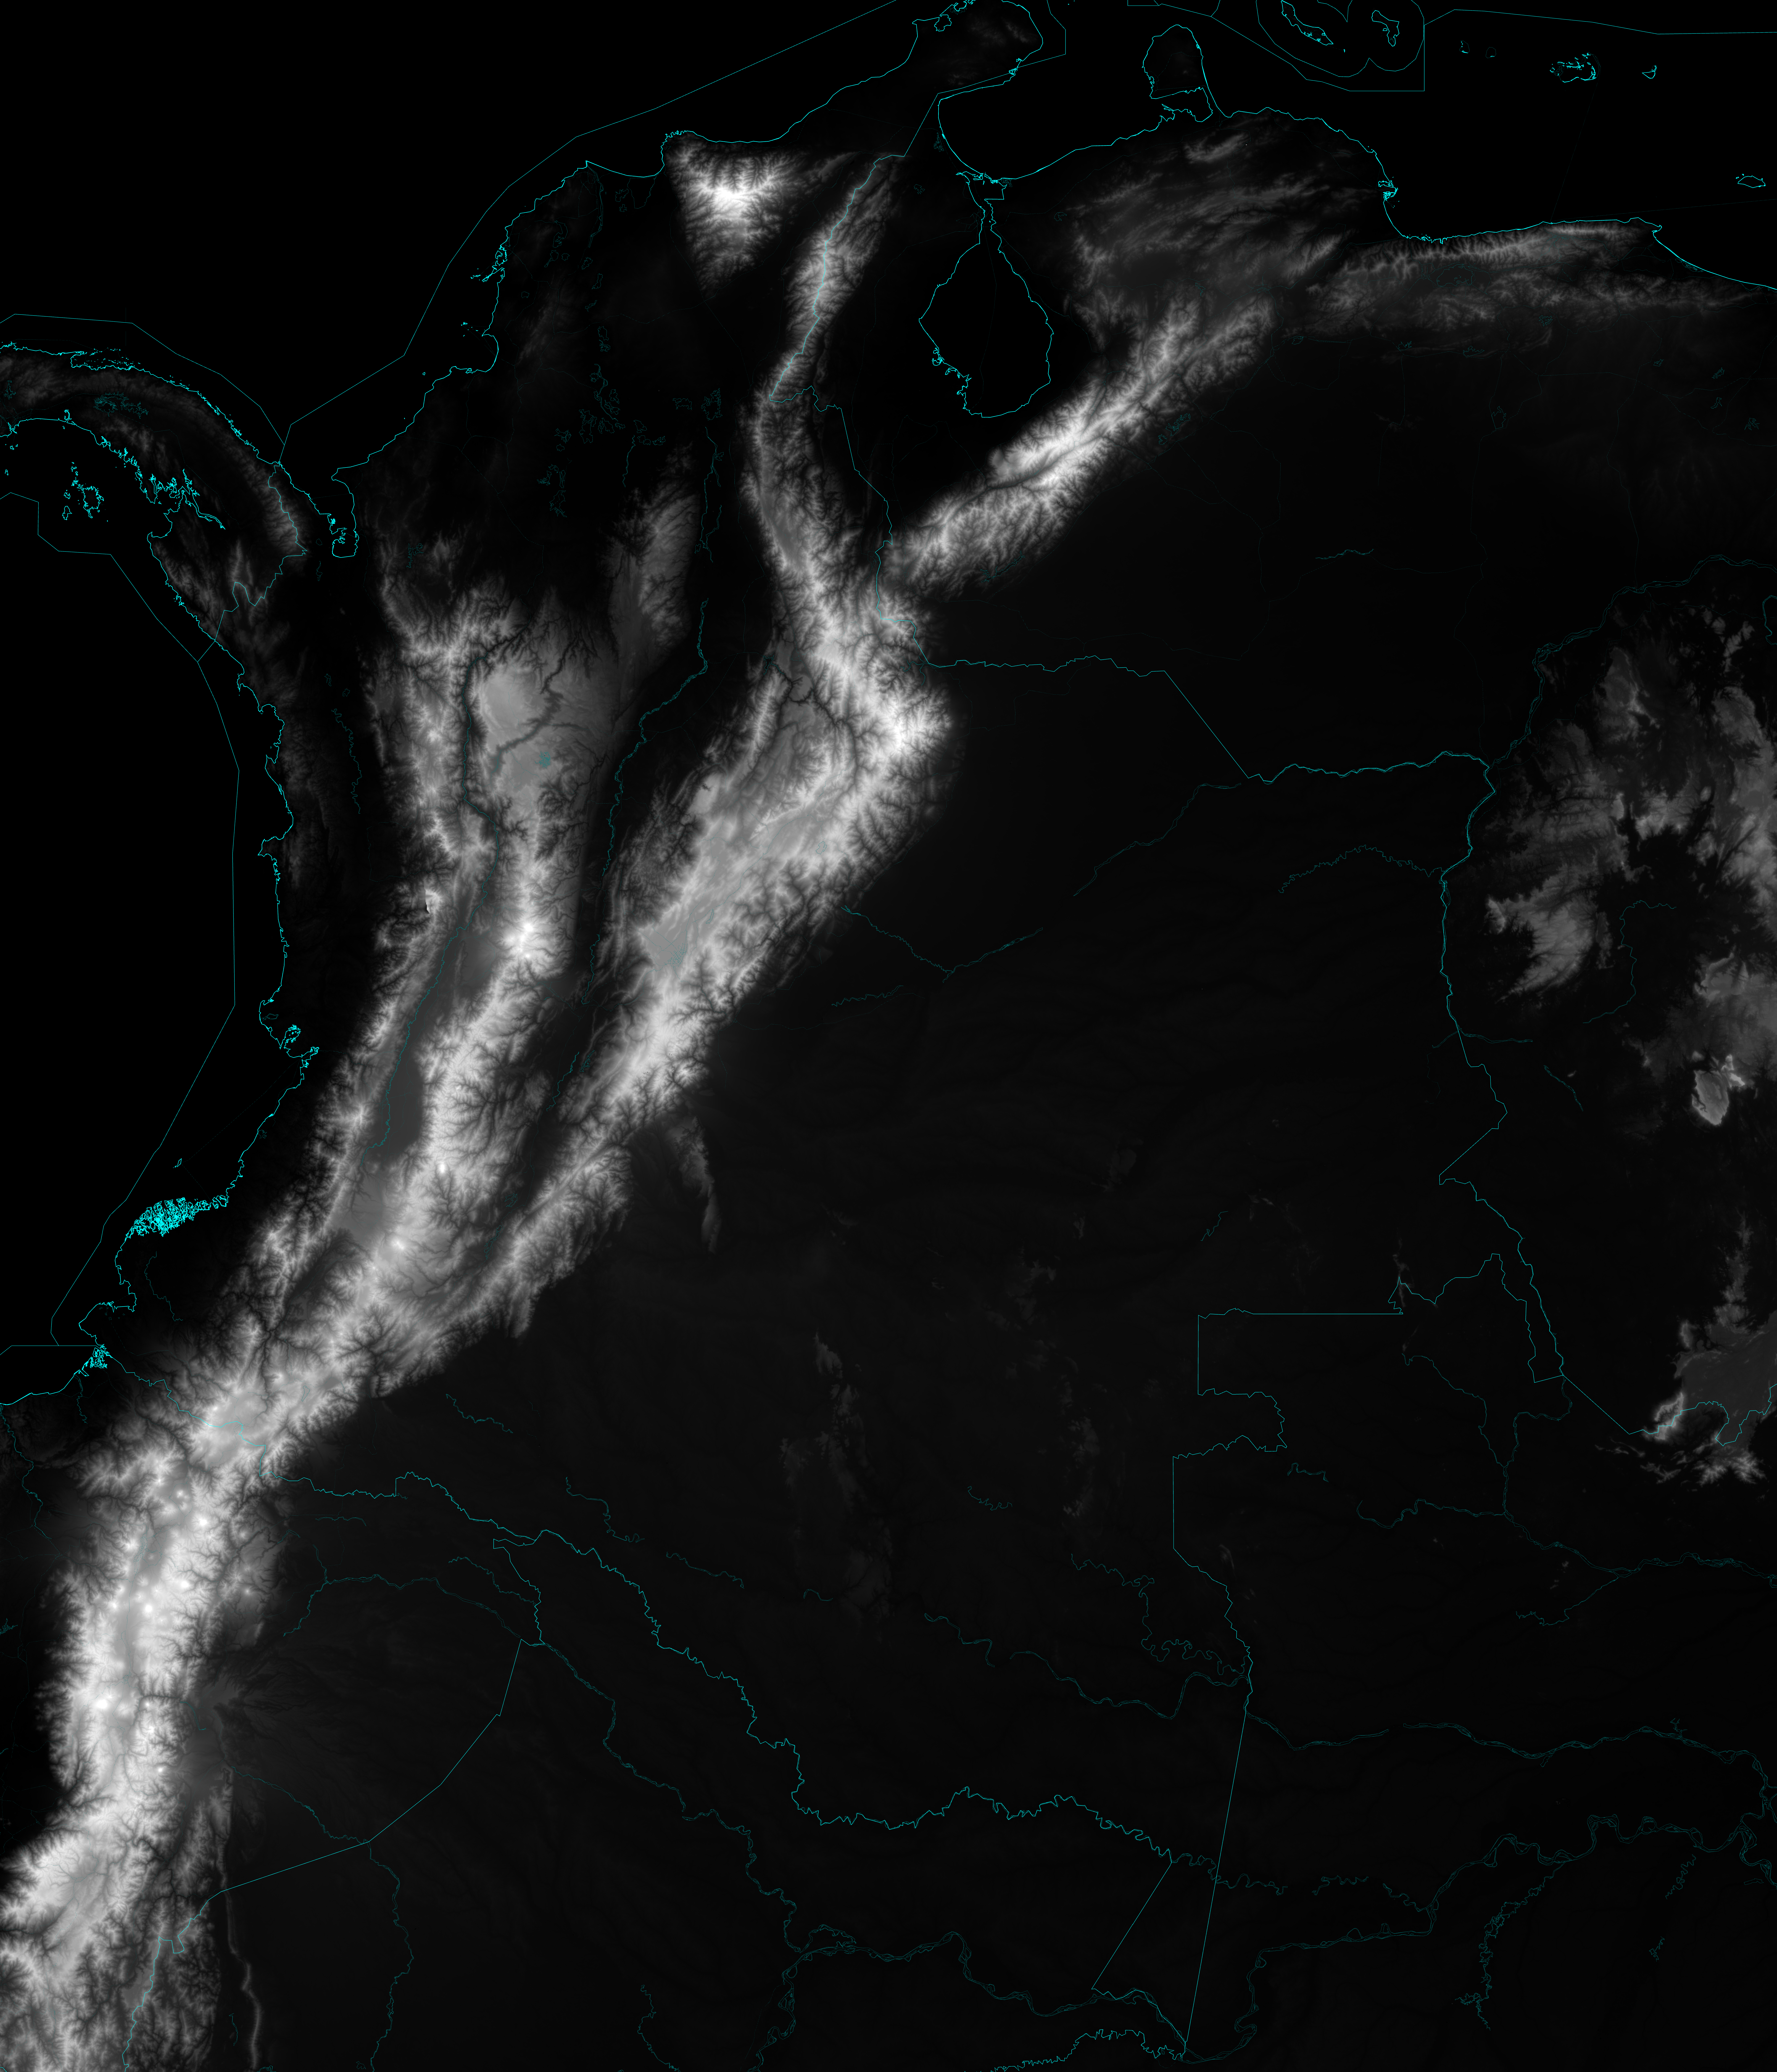
\includegraphics[width=\linewidth]{figures/mapa_alturas.png}
    \caption*{(a) Mapa de elevación en escala de grises.}
\end{minipage}\hfill
\begin{minipage}{0.45\textwidth}
    \centering
    \includegraphics[width=\linewidth]{figures/mapa_colombia_v1.jpeg}
    \caption*{(b) Modelo tridimensional generado en Blender.}
\end{minipage}
\caption{Generación del terreno mediante mapa de elevación en Blender.}
\label{fig:mapa-altura}
\end{figure}

Sin embargo, el modelo obtenido presentaba una alta densidad de polígonos, con un total de 24.5 millones de vértices, como se muestra en la Figura \ref{fig:rendimiento-terreno}.
Debido a ello, durante las pruebas se registró una tasa de cuadros por segundo (\textit{frames per second}, FPS) promedio de 25.9, valor considerablemente inferior al rango óptimo de 30 a 60 FPS recomendado para garantizar una experiencia fluida.
Este rendimiento reducido afectaba tanto el desempeño real del sistema como la percepción del usuario, generando una sensación de lentitud e inestabilidad en la simulación.
\begin{figure}[H]
\centering
\includegraphics[width=0.8\textwidth]{figures/bajo_rendimiento.jpeg}
\caption{Ejemplo del alto número de polígonos del modelo 3D que afecta el rendimiento.}
\label{fig:rendimiento-terreno}
\end{figure}

Esta situación evidenció que el uso de un modelo tridimensional completo para representar el terreno no era una solución óptima, especialmente considerando los requerimientos de eficiencia y fluidez del entorno de simulación.
Por ello, se decidió implementar un método alternativo, que anteriormente desconocíamos, de generación del mapa, con el fin de mejorar la eficiencia y el rendimiento general del entorno virtual.
\subsubsection{Vías}
En un intento por optimizar el proceso de generación del trazado ferroviario, se exploró inicialmente la posibilidad de representar las vías mediante la conexión de puntos y segmentos rectos.
Este enfoque, aunque sencillo en su concepción, requería una gran cantidad de puntos para lograr una precisión adecuada en curvas y pendientes, lo cual incrementaba la complejidad del sistema y afectaba el rendimiento general.
Ante esta limitación, se consideró el uso de \textit{splines}, una técnica matemática que permite la creación de curvas suaves a partir de un conjunto reducido de puntos de control.
Las splines resultan especialmente adecuadas para la representación de vías férreas, ya que facilitan la generación de trayectorias continuas y realistas sin necesidad de definir manualmente cada punto intermedio, mejorando así tanto la precisión geométrica como la eficiencia del proceso de renderizado.
%le añadimos las columnas a los riesgos, con una nueva *tabla de de que tanto riesgo hay* y con eso definimos la columna nivel de riesgo y pues se pone la tabla entera ahora si, lo hemos puesto abierto y cerrado si ya esta hecho
%que este cerrado es que ya se soluciono o se acepto, como los de poco riesgo, que puede..... osea existen cerrados que es porque el problema es muy minimo, no es tan grave

\subsection{Refinación de la lista de riesgos}

Para mejorar la comprensión y categorizar adecuadamente los posibles riesgos presentados en la sección \textit{PONER PRIMERA SECCIÓN DONDE SE 
PRESENTA EL DOC DE RIESGOS}, se diseñó un sistema de evaluación de riesgos compuesto por dos tablas complementarias.
En primer lugar, se definió un rango de niveles de riesgo, donde se definen los valores numéricos del 1 al 5 que representan la magnitud del impacto y la probabilidad de ocurrencia de un evento.
En esta escala, el valor 1 indica una afectación mínima o poco probable, mientras que el valor 5 corresponde a un evento con consecuencias críticas o de alta probabilidad, tal como se explica en la Figura \ref{fig:linea_impacto_probabilidad}.
\begin{figure}[H]\centering
  \includegraphics[width=\linewidth]{figures/linea de impacto-probabilidad.png}
  \caption{Rango de riesgos y Probabilidad.
Fuente: Propia}
  \label{fig:linea_impacto_probabilidad}
\end{figure}

En segundo lugar, se desarrolló una tabla general de riesgos, en la que se registran los posibles problemas identificados durante el proyecto.
Esta tabla incluye los campos Descripción (donde se detalla el problema detectado), Causa, Impacto, Probabilidad, Nivel de riesgo (calculado como el producto del impacto con la probabilidad), Plan de acción (estrategias o medidas a tomar) y Estado (donde se especifica si el riesgo permanece abierto o ya ha sido cerrado).
En la tabla \ref{tab:matriz-riesgos} se muestra el artefacto entregado.

Hay que aclarar que, algunos riesgos se mantuvieron abiertos incluso hasta el final del desarrollo del proyecto.
Esto se debe a que se consideró que el nivel de riesgo era suficientemente bajo como para evitar gastar recursos en solucionarlo.
\begin{landscape}
\begin{longtable}{|c|L{2.8cm}|L{2.8cm}|c|c|c|L{3.2cm}|c|}
\caption{Matriz de riesgos del proyecto}\label{tab:matriz-riesgos} \\
\hline
\multicolumn{1}{|c|}{\textbf{No. Ref}} &
\multicolumn{1}{c|}{\textbf{Descripción}} &
\multicolumn{1}{c|}{\textbf{Causa}} &
\multicolumn{1}{c|}{\textbf{Impacto}} &
\multicolumn{1}{c|}{\textbf{Probabilidad}} &
\multicolumn{1}{c|}{\textbf{Nivel de Riesgo}} &
\multicolumn{1}{c|}{\textbf{Plan de acción}} &
\multicolumn{1}{c|}{\textbf{Estado}} \\
\hline
\endfirsthead

\hline
\multicolumn{1}{|c|}{\textbf{No.
Ref}} &
\multicolumn{1}{c|}{\textbf{Descripción}} &
\multicolumn{1}{c|}{\textbf{Causa}} &
\multicolumn{1}{c|}{\textbf{Impacto}} &
\multicolumn{1}{c|}{\textbf{Probabilidad}} &
\multicolumn{1}{c|}{\textbf{Nivel de Riesgo}} &
\multicolumn{1}{c|}{\textbf{Plan de acción}} &
\multicolumn{1}{c|}{\textbf{Estado}} \\
\hline
\endhead

R1 & El modelo del terreno del mapa de Colombia está mal optimizado & El uso de modelo 3D genera una sobrecarga en la memoria gráfica & 4 & 4 & 16 & Realización de un terreno formal de Unity sin usar Blender.
Carga de terreno por bloques. & Cerrado \\ \hline
R2 & La cámara del jugador puede atravesar el terreno.
& La cámara no está programada para evadir o chocar con el mapa.
& 2 & 5 & 10 & Implementación de una función para aplicar una colisión de cámara con el terreno y evitar el paso.
& Abierto \\ \hline
R3 & Las vías se generan de manera poco natural e inconexa.
& Uso de puntos y rectas para la asignación de vías & 5 & 4 & 20 & Cambiar a uso de spline.
& Cerrado \\ \hline
R4 & Terreno con parches o incoherencias.
& El DEM utilizado está con ciertos datos erróneos o vacíos.
& 2 & 3 & 6 & Cambiar de DEM o arreglar los parches haciendo uso de algoritmos.
& Cerrado \\ \hline
R5 & Textura de vías solapando suelo en plano.
& Vía colocada en el punto exacto donde está el terreno, generando solapamiento & 1 & 2 & 2 & Mover las vías generadas una pequeña distancia hacia arriba & Cerrado \\ \hline
R6 & Las vías no permiten al tren dar vueltas en un circuito cerrado.
& Spline no cerrado & 2 & 3 & 6 & Añadir que el circuito detecte cuando se colocan vías cerca al punto inicial, y de ser así cierre el circuito & Cerrado \\ \hline
R7 & Dificultad para representar todos los ríos y lagos de Colombia en el mapa.
& Colombia tiene una gran densidad de elementos hidrológicos, que superan la capacidad de representación fiel en el terreno del videojuego.
& 4 & 4 & 16 & Definir criterios de selección: incluir solo ríos principales y lagos mayores.
& Abierto \\ \hline
R8 & Las vías atraviesan montañas & La generación de vías no interpola dichas alturas & 3 & 4 & 12 & Modificar la función de generación de vías, para que, cuando la vía atraviese el terreno, genere un túnel en la zona atravesada.
& Cerrado \\ \hline
R9 & Estadísticas de las locomotoras no son leídas correctamente & Estadísticas guardadas en los GameObject hijos de la Locomotora & 4 & 2 & 8 & Unificar la lógica y estadísticas de las distintas locomotoras en el GameObject padre Locomotora & Cerrado \\ \hline
R10 & HUD no muestra la vida actual del tren al hacer cambio de locomotora & Dato de vida y estadísticas no leído después del cambio & 2 & 2 & 4 & Crear una función para reiniciar las estadísticas del tren & Cerrado \\ \hline
R11 & Modelos 3D de los trenes y 
ciudades se ven a escalas diferentes & Escalas y rotaciones no aplicadas correctamente en Blender & 1 & 3 & 3 & Aplicar escalas y rotaciones a los modelos 3D de los trenes y ciudades & Cerrado \\ \hline
R12 & Shaders incompatibles y LOD's mal configurados.
& Unity tiene valores por defecto en las generaciones de terreno que no siempre es compatible entre shaders y capas de niveles de detalle.
& 3 & 3 & 9 & Testear y ajustar shaders, URP, en diferentes escenarios, hasta llegar a la configuración correcta.
& Cerrado \\ \hline
R13 & El videojuego puede andar en muy bajos FPS en los equipos de cómputo de los usuarios.
& Al desarrollar el proyecto en equipos con especificaciones mayores a la media, se omite algunos aspectos de optimización.
& 5 & 3 & 15 & Investigar las especificaciones de los equipos donde se realizará la prueba y reevaluar riesgos.
& Abierto \\ \hline
\end{longtable}
\end{landscape}

%al final si van las HU completas, 
%añadir una fase extra para colocar el diagrama de actividades inicial (el diagrama de actividades es mental)y el diagrama de componentes *el UML grande q urbano ni miró*, hay que explicarlo por partes por lo gigante

Finalmente, se asignaron a las historias de usuario la técnica de priorización MoSCoW, enfocando el proyecto en lo más valioso y viable.
Clasifica en: Must have (imprescindible), Should have (importante), Could have (deseable si hay recursos) y Won’t have (no se hará por ahora).
Así mismo, se estableció la variable de cumplimiento, con valores comprendidos entre 0 y 1, donde 0 indica que la actividad no se ha iniciado y 1 que ha sido completada en su totalidad, este no fue agregado en la Tabla \ref{tab:HU-epica} ya que todos fueron cumplidos.
Por último, se definió el nivel de complejidad, con una escala de 1 a 5, en la cual 1 corresponde a tareas de baja dificultad y 5 a aquellas de mayor complejidad.
\begin{landscape}
\begin{longtable}{|M{1.2cm}|M{1.8cm}|L{8cm}|M{2.2cm}|M{2cm}|}
\caption{Tabla final de historias de usuario.} \label{tab:HU-epica} \\
\hline
\multicolumn{1}{|c|}{\textbf{ÉPICA}} &
\multicolumn{1}{c|}{\textbf{CÓDIGO}} &
\multicolumn{1}{c|}{\textbf{HISTORIA DE USUARIO}} &
\multicolumn{1}{c|}{\textbf{PRIORIZACIÓN}} &
\multicolumn{1}{c|}{\textbf{COMPLEJIDAD}} \\ \hline
\endfirsthead

\hline
\multicolumn{1}{|c|}{\textbf{ÉPICA}} &
\multicolumn{1}{c|}{\textbf{CÓDIGO}} &
\multicolumn{1}{c|}{\textbf{HISTORIA DE USUARIO}} &
\multicolumn{1}{c|}{\textbf{PRIORIZACIÓN}} &
\multicolumn{1}{c|}{\textbf{COMPLEJIDAD}} \\ \hline
\endhead

\hline
\multicolumn{5}{r}{\textit{Continúa en la siguiente página}} \\
\endfoot

\hline
\endlastfoot

1 & HU1  & Como jugador, quiero ver una pantalla de selección de niveles para elegir cuál jugar.
& M & 2 \\ \hline
1 & HU2  & Como jugador, quiero que al empezar un nivel, se me presente una pantalla de contrato que detalle el presupuesto, los objetivos y los posibles desafíos.
& M & 1 \\ \hline
2 & HU3  & Como jugador, quiero poder mover la cámara (panorámica) por el mapa para explorar el terreno.
& M & 1 \\ \hline
2 & HU4  & Como jugador, quiero poder acercar y alejar la vista (zoom) para ver el mapa con diferentes niveles de detalle.
& M & 1 \\ \hline
2 & HU5  & Como jugador, quiero ver las delimitaciones políticas y ríos.
& M & 3 \\ \hline
2 & HU6  & Como jugador, quiero ver un terreno del nivel a jugar.
& M & 4 \\ \hline
2 & HU7  & Como jugador, quiero poder rotar la cámara para observar el terreno desde distintos ángulos.
& S & 1 \\ \hline
2 & HU8  & Como jugador, quiero poder activar una capa de vista topográfica para entender el relieve del terreno.
& C & 5 \\ \hline
3 & H10  & Como jugador, quiero poder construir un tramo de vía férrea entre dos puntos.
& M & 2 \\ \hline
3 & H11  & Como jugador, quiero poder eliminar un tramo de vía férrea para rediseñar mis rutas.
& M & 1 \\ \hline
3 & HU12 & Como jugador, quiero que se pueda construya un puente o valles.
& M & 4 \\ \hline
3 & HU13 & Como jugador, quiero que se construya automáticamente un túnel si mi vía férrea atraviesa una montaña.
& M & 4 \\ \hline
3 & HU14 & Como jugador, quiero poder construir estaciones en puntos específicos de la vía para definir los puntos de inicio y fin del ciclo.
& M & 3 \\ \hline
3 & HU15 & Como jugador, quiero que la interfaz muestre mi presupuesto actual en todo momento para controlar mis gastos de construcción.
& M & 2 \\ \hline
3 & HU16 & Como jugador, quiero poder deshacer mi última acción de construcción para corregir un error rápidamente.
& S & 2 \\ \hline
4 & HU17 & Como jugador, tras diseñar la ruta, quiero acceder a un menú para seleccionar y comprar la locomotora que usaré.
& M & 3 \\ \hline
4 & HU18 & Como jugador, quiero poder añadir vagones específicos (pasajeros, carga) a mi locomotora para cumplir los requisitos del contrato.
& M & 2 \\ \hline
4 & HU19 & Como jugador, quiero que el menú de selección me muestre las locomotoras de la ruta que diseñé.
& C & 2 \\ \hline
5 & HU20 & Como jugador, durante la simulación, quiero ver una alerta o efecto visual cuando un tren está sufriendo daños al pasar por una zona de evento.
& M & 2 \\ \hline
5 & HU21 & Como jugador, quiero que el botón de "Hacer Testeo" me informe si me falta algún requisito para iniciar la simulación.
& S & 3 \\ \hline
5 & HU22 & Como jugador, quiero tener la opción de volver a la fase de construcción después de un testeo para modificar mis rutas antes de la evaluación final.
& S & 1 \\ \hline
6 & HU23 & Como jugador, al finalizar un nivel, quiero ver una pantalla de puntuación que califique mi desempeño.
& M & 3 \\ \hline
6 & HU24 & Como jugador, quiero que mi puntuación final considere la rentabilidad (costo total vs. valor del contrato).
& M & 3 \\ \hline
6 & HU25 & Como jugador, quiero que mi puntuación final considere la durabilidad (estado final de mis trenes y vías tras la simulación).
& M & 3 \\ \hline
6 & HU26 & Como jugador, quiero que mi puntuación final considere la eficiencia (tiempo que tardó el tren en completar el ciclo).
& S & 3 \\ \hline
6 & HU27 & Como jugador, quiero ver un informe detallado que desglose mi puntuación final para entender cómo mejorar.
& S & 3 \\ \hline
7 & HU28 & Como jugador, quiero que se desbloqueen nuevos niveles en el menú de selección tras completar el contrato actual.
& M & 2 \\ \hline
8 & HU29 & Como jugador, quiero que Don Raíl me presente el contrato al inicio de cada nivel con un diálogo breve, para darme un objetivo narrativo y contexto histórico sobre la región.
& S & 3 \\ \hline
8 & HU30 & Como nuevo jugador, quiero que Don Raíl me guíe a través de un tutorial interactivo en el primer nivel, para aprender las mecánicas del juego de una forma amigable y contextual.
& S & 4 \\ \hline
8 & HU31 & Como jugador, quiero que Don Raíl me dé una advertencia contextual si construyo una vía con una pendiente muy pronunciada o una curva muy cerrada, para que pueda corregir errores de ingeniería antes del testeo.
& S & 4 \\ \hline
8 & HU32 & Como jugador, quiero que al seleccionar una estación o ciudad importante, aparezca un ícono de Don Raíl que pueda clickear para escuchar un dato histórico sobre la importancia ferroviaria de ese lugar.
& S & 4 \\ \hline
8 & HU33 & Como jugador, quiero escuchar o leer un breve comentario de Don Raíl cuando un tren sufre un evento durante la simulación, para aumentar la inmersión.
& S & 3 \\ \hline
8 & HU34 & Como jugador, quiero que Don Raíl comente sobre mi puntuación final, celebrando el éxito con emoción o dándome un consejo en caso de fallar para que la evaluación se sienta más personal.
& S & 2 \\ \hline
8 & HU35 & Como jugador, quiero que durante las pantallas de carga, aparezcan anécdotas cortas o "dichos" de Don Raíl sobre la vida en el ferrocarril, para enriquecer el mundo del juego y aprovechar los tiempos de espera.
& M & 2 \\ \hline
6 & HU36 & Como administrador, quiero adquirir y guardar metadatos de los jugadores en una base de datos para poder generar informes.
& M & 3 \\ \hline

\end{longtable}
\end{landscape}



\section{Implementación}
% (Completar) vendria a ser implementacion
poner el tablero kanban, hay que inventarse que hizo cada uno pq no hay registro, tiene que tener semanas, inventadas si no recordamos / tipo semana 1, semana 2, semana 3-5, semana 6 a 7 y asi hasta que la columna de finalizado este completa.
mejor dicho de la semana tal a tal se hizo esto, de esta a esta se hizo esto.
poner entre semanas y narrar un poco el progreso, sucedieron estos problemas, decidimos hacer ciertos cambiso a tal cosa

hay mas libertad la vdd, asi q esto es un comodin *BALATRO REFERENCIA*

estaria bien colocar el diagrama de componentes aca si terminado final y explicado a detalle

\section{Pruebas}
% (Completar) vendria a ser evaluacion

publicarlo en internet

obtener resultados de envuesta de jugadores

analizar los resultados, nadie jugo el 3 nivel, pirobos

*unificar actividades* A1